\documentclass[UTF8]{ctexart}
\usepackage{amsfonts}
\usepackage{amsmath}
\usepackage{amssymb}
\usepackage{amsthm}
\usepackage{booktabs}
\usepackage{color}
\usepackage{courier}
\usepackage{float}
\usepackage{geometry}
\usepackage{graphicx}
\usepackage{graphics}
\usepackage{hyperref}
\usepackage{listings}

\geometry{left=2.54cm,right=2.54cm,top=2.18cm,bottom=3.18cm}
\graphicspath{{./img/}}

\newcommand{\red}{\textcolor[rgb]{1.00,0.00,0.00}}

\begin{document}

\title{\textbf{HRPT数字卫星云图信号接收}}
\author{无44 \ 姜宏伟 \ 2014011041\\
        无46 \ 杨志坚 \ 2014011183\\
        无46 \ 严靖凯 \ 2014011192\\
        无46 \ 黄秀峰 \ 2014011193\\
        无48 \ 黄佳新 \ 2014011248}
\date{}
\maketitle

\section{背景与思路}

卫星云图接收是电子系统设计中的一个经典项目。在传统的卫星云图信号接收中,人们通常选择接收美国国家海洋和大气局(NOAA)于20世纪中期发射的气象卫星NOAA-15,16,17

美国国家海洋和大气局(NOAA)与20世纪中期发射的气象卫星NOAA-15,16,17等由于没有采用加密编码,且距地面较近,较便于接收。该卫星的发送APT信号,其下行频率为137.7MHz。该频率的信号可以通过软件无线电(SDR)直接接收与解码,并利用WXtoImg等软件直接显示。这是目前大多数卫星云图信号接收所采用的信号。

同时,该卫星也发送1.7025GHz的HRPT信号,我们计划对这一信号进行接收。但由于该频率较高,难以直接用SDR直接接收。我们考虑借助东主楼顶闲置的卫星接收天线进行接收。我们已前往东主楼顶对天线进行了初步考察与清理。


\section{系统框架}

\section{HRPT信号接收与处理}

\section{放大电路设计}

\section{使用信号发生器模拟发送}

本次实验使用SFU信号源作为信号发生器,使用WinIQSIM和IQWizard处理数据生成.wv文件用于信号源生成信号,具体流程如下。

\subsection{用Matlab处理数据生成mat文件}

首先用Matlab处理我们要发送的数据,生成需要发送的I、Q两路信号数组(数值在-1至1之间),将数据保存为single类型(注意,如果不保存single类型,IQWizard在读取时会出错)。最后通过$$save('data.mat','-v6',I,Q)$$将数据存储为mat文件

\subsection{用WinIQSIM和IQWizard生成wv文件}

利用WinIQSIM和IQWizard可以将mat文件转化为信号源可读取的mv文件。

首先利用端口通信连接WinIQSIM和IQWizard

\begin{figure}[H]
        \centering
        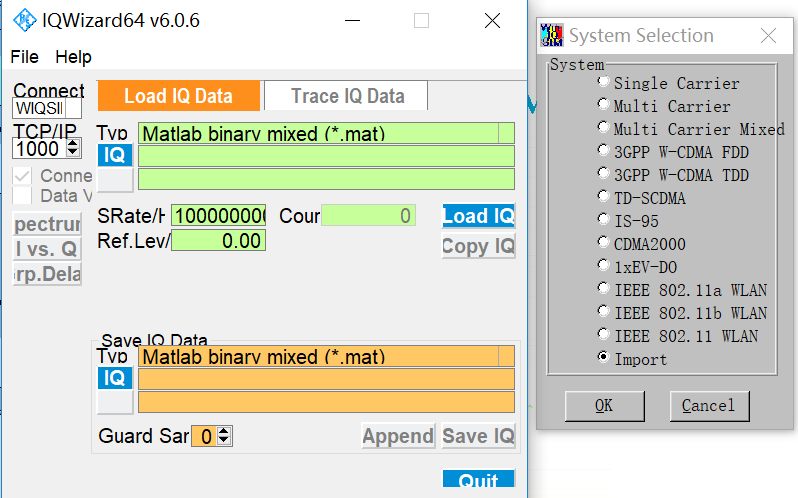
\includegraphics[width=\textwidth]{images//connect.png}
\end{figure}

将mat文件导入到IQWizard中

\begin{figure}[H]
        \centering
        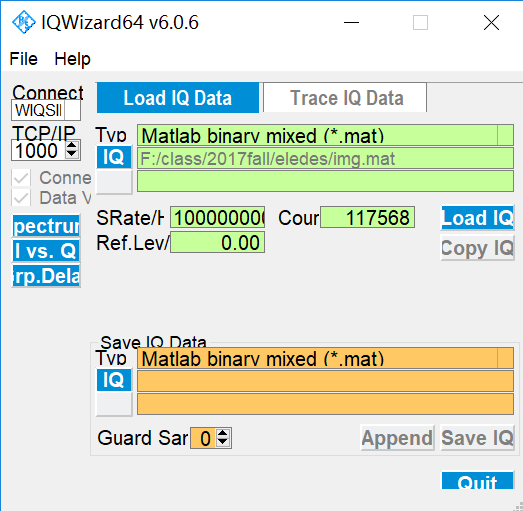
\includegraphics[width=\textwidth]{images//loadmat.png}
\end{figure}

将数据从IQWizard传输到WinIQSIM

\begin{figure}[H]
        \centering
        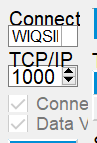
\includegraphics[width=0.5\textwidth]{images//transform.png}
\end{figure}

利用WinIQSIM将数据导出为SFU可读取的wv文件

\begin{figure}[H]
        \centering
        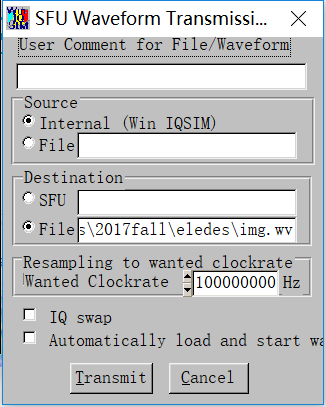
\includegraphics[width=\textwidth]{images//getwv.png}
\end{figure}

\subsection{使用SFU信号源发送信号}

选择SIGNAL SOURCE为ARB

\begin{figure}[H]
        \centering
        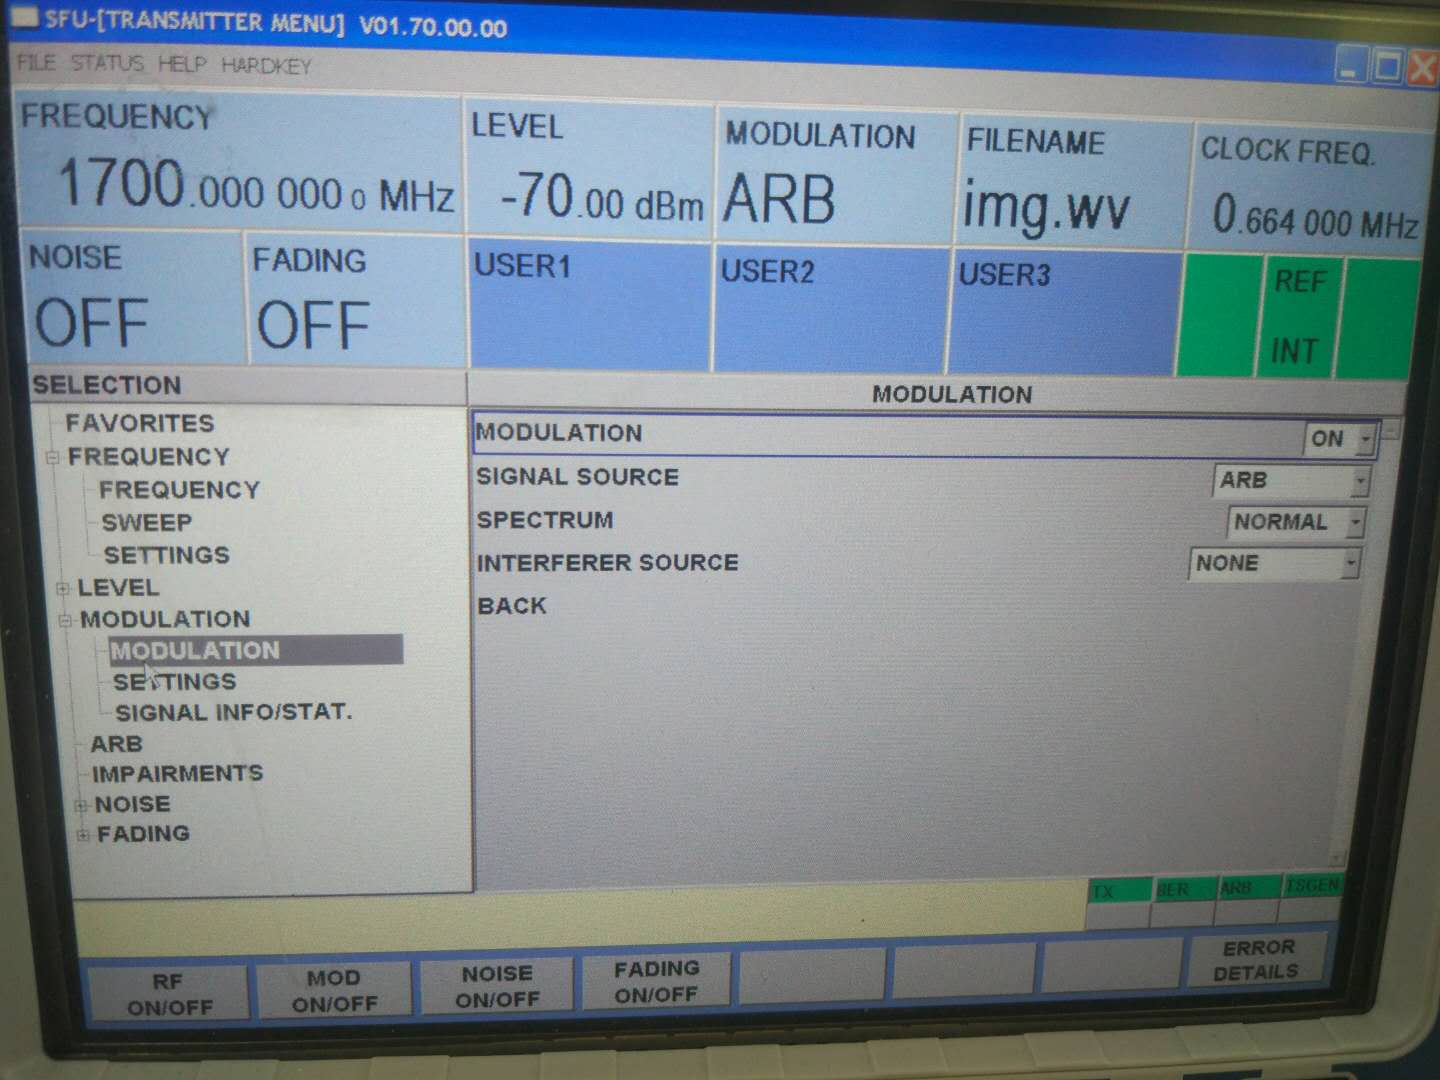
\includegraphics[width=\textwidth]{images//setARB.jpg}
\end{figure}

导入wv文件

\begin{figure}[H]
        \centering
        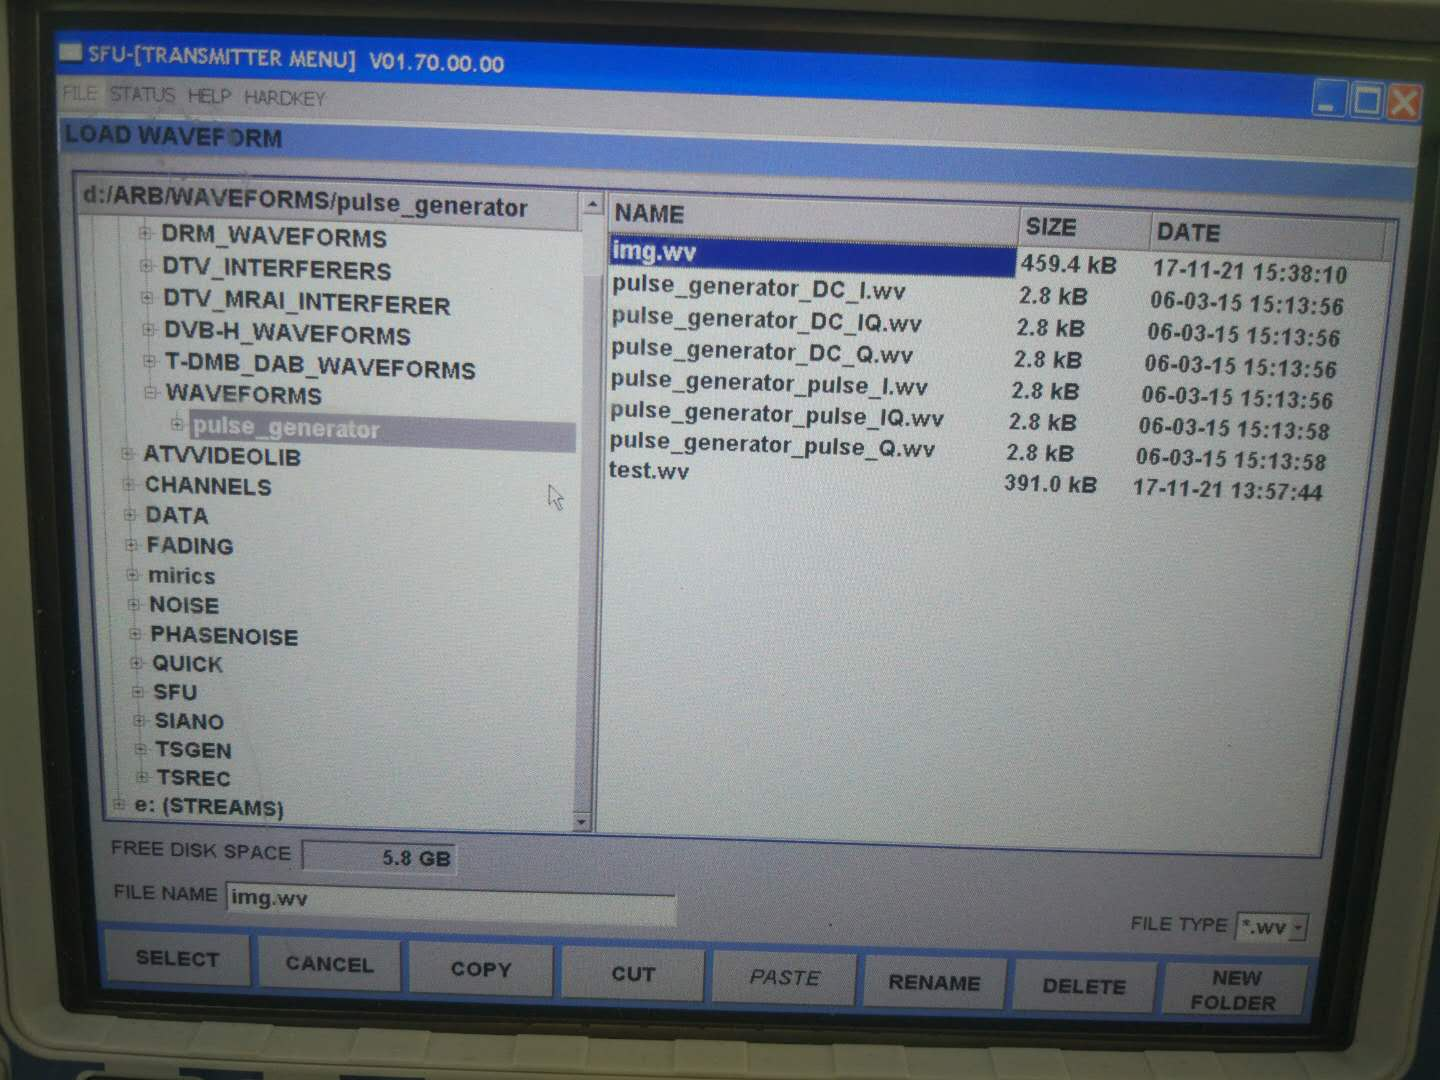
\includegraphics[width=\textwidth]{images//loadwv.jpg}
\end{figure}

选择载波频率

\begin{figure}[H]
        \centering
        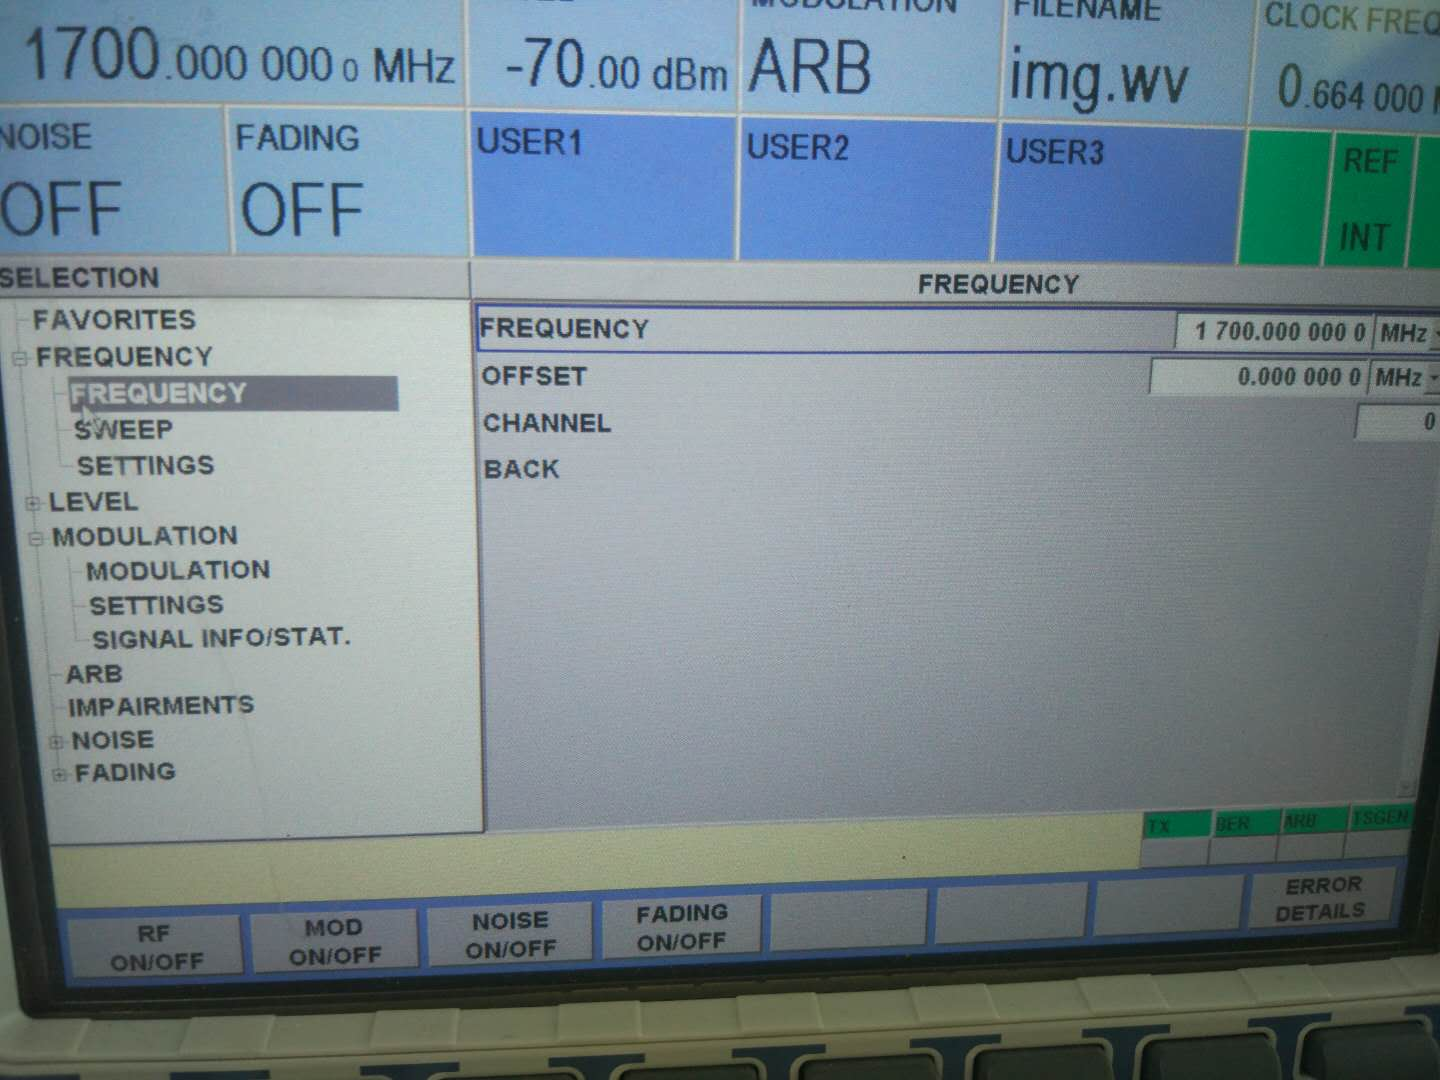
\includegraphics[width=\textwidth]{images//setfreq.jpg}
\end{figure}

设置成功后,会循环发送wv文件中的信号

\section{测试结果}

\section{分析与讨论}


\end{document} 